\documentclass[a4paper,oneside,openright,11pt]{book}

\usepackage[T1]{fontenc}
\usepackage{lmodern}
\usepackage{graphicx}
\usepackage[utf8]{inputenc}
\usepackage[ngerman]{babel}
\usepackage{listings}
\usepackage{amssymb}
\usepackage{amsmath}
\usepackage{url}
\def\UrlBreaks{\do\/\do-}
\usepackage[hidelinks]{hyperref}
\usepackage{xspace}
\usepackage{csquotes}
\usepackage{booktabs}
\usepackage{microtype}
\usepackage{epstopdf}

\setlength{\emergencystretch}{3em}
\usepackage{etoolbox}
\apptocmd{\thebibliography}{\raggedright}{}{}

\hyphenpenalty=5000
\tolerance=1000

\newcommand{\stdScaleFactor}{0.45}

% Finding-Hervorhebung im Klünder-Stil
\newcommand{\finding}[2]{%
  \medskip\noindent\textbf{Finding #1:} #2\medskip%
}

\usepackage{sethesis}

\unilogo{
\includegraphics[width=5cm]{FHDW-Logo.eps}}
\fachgebiet{}
\institut{}
\fachbereich{}

\author{Mattis Dennhardt, Arun Dylan Gopala, Alex Haase,\\Viktor Lind, Darko Marjanovic, Benedikt Racette}
\title{Speedrunning-Weltrekord-Analyse}
\englishtitle{Speedrunning World Record Analysis}
\ort{Hannover}
\thesistype{Projektarbeit}
\datum{17. Mai 2026}

\begin{document}

\frontmatter

\maketitle

\clearpage
\input{affirmation}

\clearpage
\chapter*{Zusammenfassung}

Diese Ausarbeitung untersucht den Verlauf von Speedrunning-Weltrekorden auf der Plattform \textit{speedrun.com}. Auf Basis von 876~Weltrekord-Datenpunkten aus 17~Spielen in sieben~Genres werden drei Forschungsfragen beantwortet: (1)~Wie stark hat sich die Bestzeit prozentual je Spielkategorie reduziert? (2)~Gibt es einen Sättigungspunkt, ab dem weitere Verbesserungen abnehmen? (3)~Welchen Einfluss haben externe Beschleuniger auf die Rekordentwicklung --- konkret: setzt ein Durchbruch die Abflachungsrate zurück~(3a), ist der Tool-Einfluss im Datensatz messbar~(3b), und wie lange hält ein Weltrekord im Mittel je Genre und Jahrzehnt~(3c)?

Als Methoden kommen nichtparametrische Tests (Kruskal-Wallis, Mann-Whitney~U), der Kaplan-Meier-Schätzer für Überlebenszeitanalysen sowie AIC-basierter Modellvergleich mit anschließendem Chow-Test auf Strukturbrüche zum Einsatz.

Die Ergebnisse zeigen erhebliche Unterschiede in der Zeitreduktion zwischen Spielen (\textbf{9,4~\% bis 99,5~\%}). Verbesserungsdynamiken weisen universelle Strukturbrüche auf (Chow-Test, \textbf{alle 17~Spiele} signifikant), was auf initiale Optimierungsschübe durch frühe Community-Aktivität hindeutet. Nach einem Durchbruch-Ereignis zeigen \textbf{5 von 6} auswertbaren Spielen ein klares Plateau ($\phi < 0{,}5$); Durchbrüche setzen die Abflachungsrate demnach nicht zurück, sondern leiten eine Konsolidierungsphase ein. Für \textbf{2 von 17~Spielen} ist ein stabiler Modell-Grenzwert bestimmbar: \textit{Half-Life~2} hat \textbf{95,5~\%} der möglichen Reduktion bis zum Modell-Floor erreicht, \textit{Pokémon Red/Blue} \textbf{82,5~\%}. Die Lebensdauer von Weltrekorden unterscheidet sich signifikant zwischen Genres ($\mathbf{H(6) = 43{,}82}$; $\mathbf{p < 0{,}001}$; $\eta^2 \approx 0{,}044$), wobei RPG-Rekorde mit einem Kaplan-Meier-Median von \textbf{52~Tagen} deutlich länger Bestand haben als Rekorde anderer Genres (Median: \textbf{7–17~Tage}).

\clearpage


\tableofcontents

\mainmatter

\chapter{Einleitung}
\label{chap:einleitung}

Speedrunning bezeichnet die Praxis, Videospiele so schnell wie möglich abzuschließen. Was ursprünglich als Nischenbeschäftigung begann, hat sich zu einer globalen Wettbewerbskultur mit eigenen Events, Kommentatoren und einer kontinuierlich wachsenden Online-Community entwickelt. Die Plattform speedrun.com fungiert dabei als zentrale Infrastruktur: Sie sammelt, verifiziert und archiviert Weltrekordversuche aus tausenden von Spielen und stellt die historischen Daten über eine öffentliche API bereit~\cite{speedruncom_api}.

Aus datenwissenschaftlicher Perspektive bieten Speedrunning-Weltrekorde ein besonders geeignetes Untersuchungsobjekt. Alle Laufzeiten werden in Sekunden gemessen und von der Community verifiziert; der Beobachtungszeitraum reicht bei einigen Spielen bis in die 1990er~Jahre zurück. Die hierarchische Datenstruktur nach Genre und Kategorie ermöglicht systematische Gruppenvergleiche. Der Verlauf von Weltrekorden lässt sich als kollektiver Optimierungsprozess interpretieren: Eine dezentrale Community entdeckt schrittweise neue Routen, Bewegungstechniken und Programmfehler (sogenannte \emph{Glitches}), die kürzere Durchläufe ermöglichen.

\section*{Forschungsfragen}

Diese Ausarbeitung untersucht anhand eines selbst erhobenen Datensatzes aus 17~Spielen in sieben~Genres drei Forschungsfragen:

\begin{enumerate}
    \item \textbf{Zeitreduktion:} Wie stark hat sich die Bestzeit prozentual je Spielkategorie reduziert, und unterscheiden sich Genres systematisch in ihren Verbesserungsraten?
    \item \textbf{Sättigung:} Folgt die Verbesserungsrate einem erkennbaren mathematischen Muster, und gibt es einen statistisch nachweisbaren Sättigungspunkt?
    \item \textbf{Lebensdauer:} Wie lange hält ein Weltrekord im Mittel, und unterscheidet sich die Lebensdauer zwischen Genres und Jahrzehnten?
\end{enumerate}

Abbildung~\ref{fig:kaos} zeigt den KAOS-Baum,\footnote{KAOS: Konzepte, Annahmen, Operationen, Struktur --- ein Modell zur Strukturierung von Forschungsfragen.} der die Beziehungen zwischen den Forschungsfragen, dem Datensatz und dem Analyseziel darstellt.

\begin{figure}[htb]
  \centering
  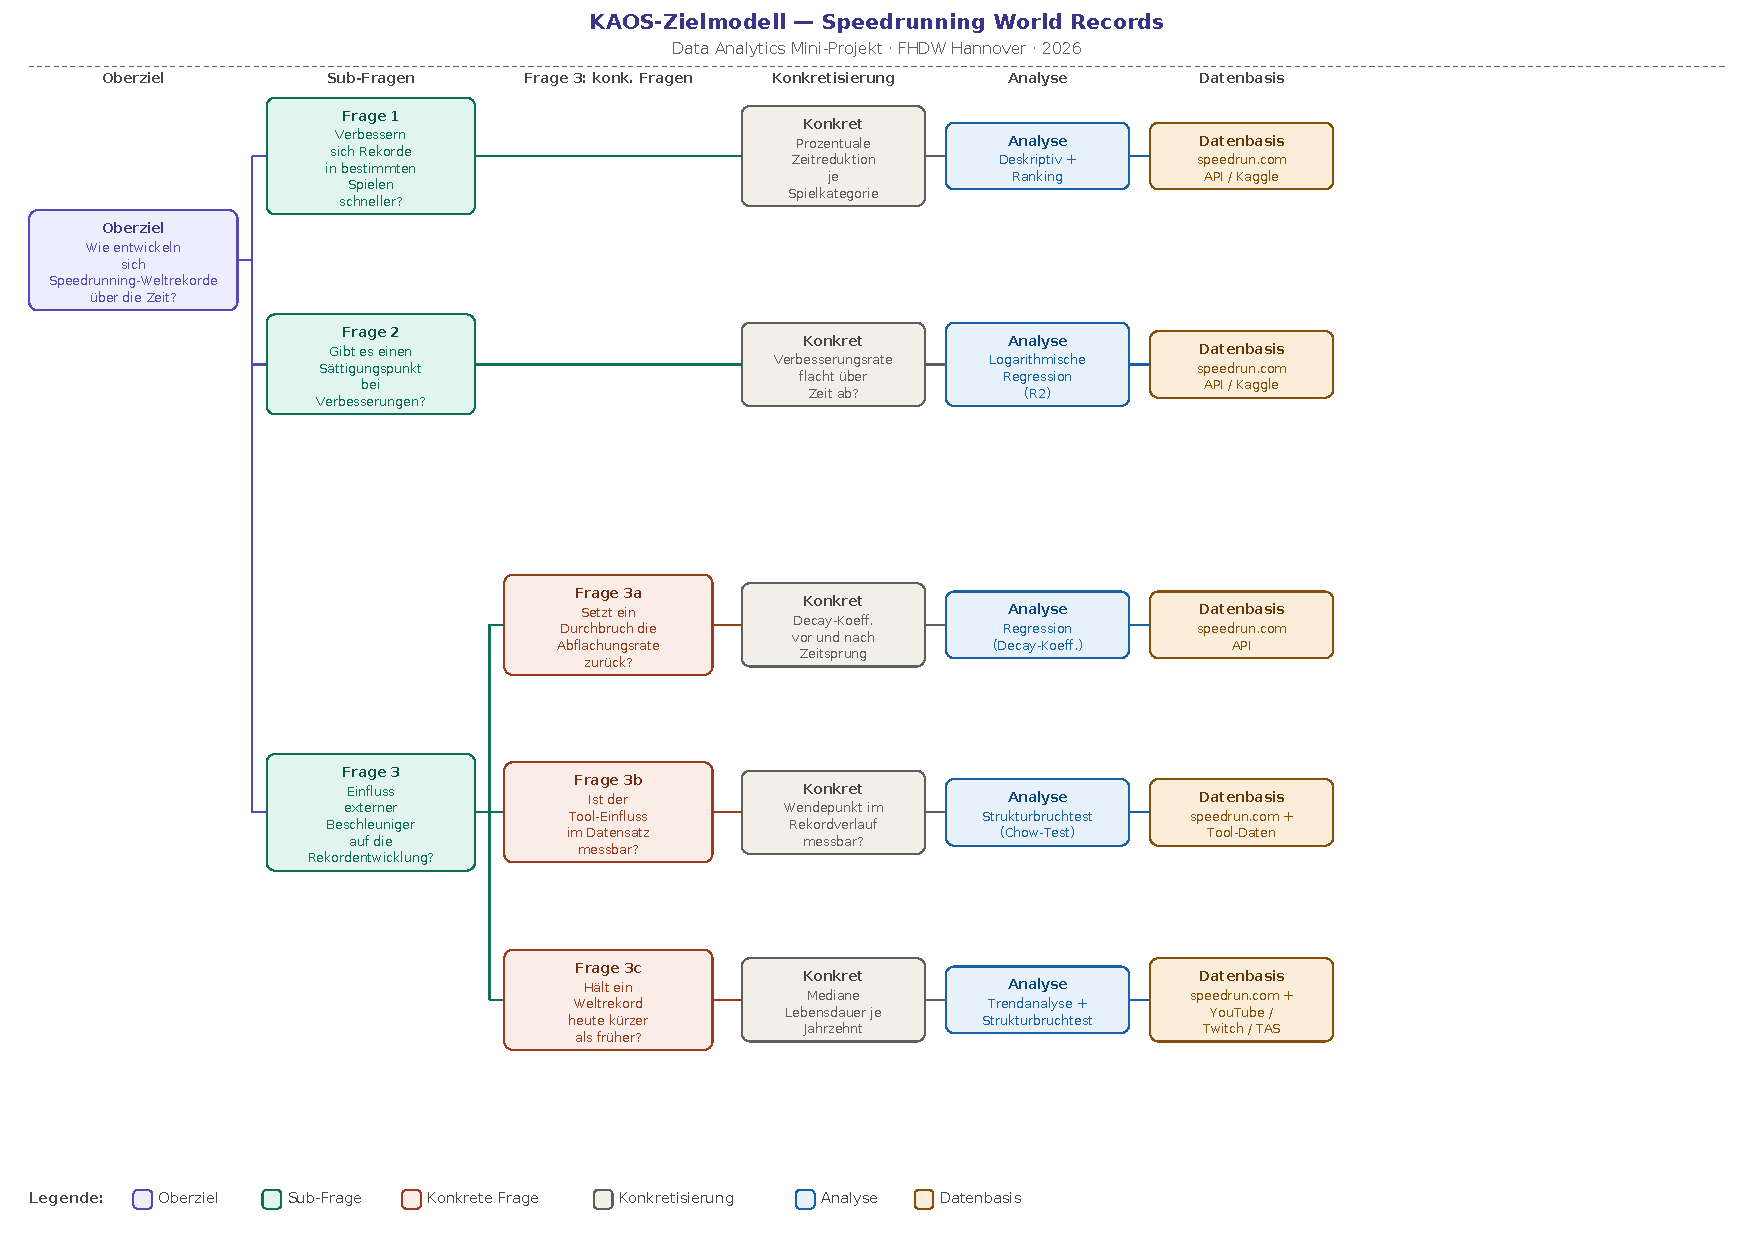
\includegraphics[width=0.55\textwidth]{contents/figures/kaos}
  \caption{KAOS-Baum der Speedrunning-Weltrekordanalyse}
  \label{fig:kaos}
\end{figure}

Die Ausarbeitung beschreibt zunächst Datenbasis und Methodik (Kap.~\ref{chap:methodik}), präsentiert die Ergebnisse zu allen drei Forschungsfragen (Kap.~\ref{chap:ergebnisse}), diskutiert Befunde und Limitationen (Kap.~\ref{chap:diskussion}) und schließt mit einem Fazit (Kap.~\ref{chap:fazit}).


\chapter{Datenbasis und Methodik}
\label{chap:methodik}

\section{Datenbeschaffung und Aufbereitung}

Die Rohdaten wurden über die speedrun.com API~v1~\cite{speedruncom_api} abgerufen. Ausgewählt wurden 17~Spiele aus sieben~Genres (Platformer, Action-Adventure, RPG, FPS, Puzzle, Sandbox, Arcade), die eine breite stilistische und zeitliche Variation abdecken (Tabelle~\ref{tab:spiele}). Alle Analysen beschränken sich auf die \emph{any\%}-Kategorie,\footnote{Any\% bezeichnet in der Speedrunning-Community den schnellsten Weg zum Spielabschluss, unabhängig vom Fertigstellungsgrad.} da diese als einzige Kategorie in allen 17~Spielen vorhanden und zwischen Spielen vergleichbar ist.

\begin{table}[htb]
  \centering
  \caption{Spieleliste nach Genre}
  \label{tab:spiele}
  \small
  \begin{tabular}{ll}
    \toprule
    \textbf{Genre} & \textbf{Spiele} \\
    \midrule
    Platformer       & Super Mario Bros., Super Mario~64, Celeste \\
    Action-Adventure & Super Metroid, Zelda: Ocarina of Time, Hollow Knight \\
    RPG              & Pokémon Red/Blue, Final Fantasy~VII \\
    FPS              & Doom~3, Quake, Half-Life~2 \\
    Puzzle           & Portal, Portal~2, The Talos Principle \\
    Sandbox          & Minecraft: Java Edition \\
    Arcade           & Pac-Man, Donkey Konga \\
    \bottomrule
  \end{tabular}
\end{table}

Die API liefert für jedes Spiel alle verifizierten Runs der gewählten Kategorie als JSON. Für Spiele mit mehr als 10.000~Runs (Minecraft) wurde die Paginierung in umgekehrter Reihenfolge wiederholt, um vollständige Daten zu erhalten. Im Bereinigungsschritt wurden unplausible Einträge entfernt (z.\,B.\ Laufzeiten von $0$~Sekunden oder Runs ohne Zeitstempel). Die bereinigten Daten umfassen fünf~CSV-Dateien mit insgesamt 842~Weltrekord-Datenpunkten für die Lebensdaueranalyse (Q3).

\section{Statistische Methoden}

\subsection*{F1 — Prozentuale Zeitreduktion (Q1)}

Die prozentuale Zeitreduktion wird definiert als:
\[
  r_i = \frac{t_{\text{first},i} - t_{\text{best},i}}{t_{\text{first},i}} \cdot 100\,\%
\]
wobei $t_{\text{first},i}$ die erste und $t_{\text{best},i}$ die aktuell beste Laufzeit im Datensatz für Spiel~$i$ ist. Zusätzlich werden die jährliche Verbesserungsrate und die Weltrekord-Dichte berechnet.

Um zu prüfen, ob Genres sich systematisch in ihren jährlichen Raten unterscheiden, wird der \textbf{Kruskal-Wallis-Test}~\cite{kruskal1952} eingesetzt. Dieser nichtparametrische Test ist eine rangskalierte Erweiterung der einfaktoriellen Varianzanalyse und setzt keine Normalverteilung der Daten voraus --- eine wichtige Eigenschaft, da Laufzeit-Daten typischerweise stark rechtsschief verteilt sind.

\subsection*{F2 — Sättigung der Verbesserungsrate (Q2)}

Für jedes Spiel wird die kumulierte Bestzeit gegen den Weltrekord-Index aufgetragen. Anschließend werden fünf Kurvenmodelle mittels nichtlinearer Regression angepasst: logarithmisch, quadratisches Polynom~(poly2), exponentieller Zerfall, Gompertz-Kurve und LOWESS (nichtparametrisch). Der Modellvergleich erfolgt über das \textbf{Akaike-Informationskriterium}~(AIC)~\cite{akaike1974}: Ein niedrigeres AIC zeigt ein besseres Verhältnis von Anpassungsgüte zu Modellkomplexität an — komplexere Modelle werden also nur bevorzugt, wenn sie die Daten deutlich besser erklären. Das Modell mit dem niedrigsten AIC je Spiel gilt als bestes Modell.

Um den Sättigungspunkt direkt nachzuweisen, wird der \textbf{Chow-Test}~\cite{chow1960} eingesetzt. Dieser prüft, ob sich die Regressionskoeffizienten vor und nach einem möglichen Strukturbruch signifikant unterscheiden ($F$-Statistik gegen $F$-Verteilung). Alle validen Trennpunkte werden durchsucht; der Trennpunkt mit der höchsten $F$-Statistik wird als Strukturbruch gemeldet.

\subsection*{F3 — Lebensdauer von Weltrekorden (Q3)}

Die Lebensdauer eines Weltrekords wird als die Anzahl Tage gemessen, die vergehen, bis er durch einen neuen Rekord abgelöst wird. Für Rekorde, die zum Analysezeitpunkt noch Bestand haben, liegt eine \emph{rechtszensierte} Beobachtung vor: Die tatsächliche Lebensdauer ist unbekannt, aber mindestens so lang wie der bisher vergangene Zeitraum.

Der \textbf{Kaplan-Meier-Schätzer}~\cite{kaplan1958} berücksichtigt diese zensierten Beobachtungen korrekt und liefert für jeden Zeitpunkt~$t$ die geschätzte Wahrscheinlichkeit, dass ein Weltrekord bis dahin noch Bestand hat. Der Median dieser Überlebensfunktion gibt an, nach wie vielen Tagen die Hälfte aller Rekorde eines Genres bereits gebrochen wurde.

Zum Vergleich der Lebensdauerverteilungen zwischen Genres wird der \textbf{Kruskal-Wallis-Test} eingesetzt. Als Effektgröße wird $\eta^2 = (H - k + 1)/(N - k)$ berechnet~\cite{cohen1988}. Paarweise Unterschiede werden mit dem \textbf{Mann-Whitney-U-Test}~\cite{mann1947} geprüft. Die Konzentration der Verbesserungsgrößen wird über den \textbf{Gini-Koeffizienten} quantifiziert ($G = 0$: vollkommen gleiche Verbesserungen, $G = 1$: eine einzelne Verbesserung dominiert alles).


\chapter{Ergebnisse}
\label{chap:ergebnisse}

\section{F1 — Prozentuale Zeitreduktion}

Tabelle~\ref{tab:q1} zeigt die prozentuale Zeitreduktion aller 17~Spiele, sortiert nach Gesamtreduktion absteigend.

\begin{table}[htb]
  \centering
  \caption{Prozentuale Zeitreduktion und jährliche Verbesserungsrate je Spiel (any\%-Kategorie)}
  \label{tab:q1}
  \small
  \begin{tabular}{llrr}
    \toprule
    \textbf{Spiel} & \textbf{Genre} & \textbf{Reduktion (\%)} & \textbf{Jährl.\ Rate (\%/a)} \\
    \midrule
    Minecraft: Java Edition         & Sandbox         & 99,5 & 8,9  \\
    The Talos Principle             & Puzzle          & 95,9 & 12,8 \\
    Portal                          & Puzzle          & 91,1 & 6,7  \\
    Hollow Knight                   & Action-Adventure& 89,8 & 12,8 \\
    Celeste                         & Platformer      & 80,2 & 9,8  \\
    Half-Life~2                     & FPS             & 75,4 & 6,2  \\
    Zelda: Ocarina of Time          & Action-Adventure& 71,2 & 15,8 \\
    Pac-Man                         & Arcade          & 69,0 & 11,2 \\
    Doom~3                          & FPS             & 61,6 & 4,8  \\
    Portal~2                        & Puzzle          & 55,2 & 4,0  \\
    Quake                           & FPS             & 47,5 & 1,8  \\
    Super Metroid                   & Action-Adventure& 41,5 & 3,1  \\
    Final Fantasy~VII               & RPG             & 34,3 & 2,9  \\
    Super Mario~64                  & Platformer      & 27,1 & 1,4  \\
    Donkey Konga                    & Arcade          & 14,9 & 2,0  \\
    Pokémon Red/Blue                & RPG             & 14,0 & 1,0  \\
    Super Mario Bros.               & Platformer      & 9,4  & 0,4  \\
    \bottomrule
  \end{tabular}
\end{table}

Auf Genre-Ebene zeigen sich deutliche Unterschiede in der mittleren Gesamtreduktion: \textit{Sandbox}~(99,5~\%), \textit{Puzzle}~(80,7~\%), \textit{Action-Adventure}~(67,5~\%) und \textit{FPS}~(61,5~\%) liegen deutlich über \textit{Arcade}~(41,9~\%), \textit{Platformer}~(38,9~\%) und \textit{RPG}~(24,2~\%). Der Kruskal-Wallis-Test auf die \emph{jährlichen Verbesserungsraten} ergibt jedoch keinen signifikanten Unterschied zwischen den sieben~Genres ($H = 6{,}24$; $p = 0{,}284$).

\finding{1}{Die prozentuale Zeitreduktion variiert stark zwischen Spielen (\textbf{9,4~\% bis 99,5~\%}). Spiele mit kurzer Spielzeit oder vielen nutzbaren Programmfehlern (\textit{Minecraft}, Puzzle-Spiele) erzielen die höchsten Reduktionen.}

\finding{2}{Ein Kruskal-Wallis-Test auf die jährlichen Verbesserungsraten zeigt keinen statistisch signifikanten Unterschied zwischen Genres ($\mathbf{H = 6{,}24}$; $\mathbf{p = 0{,}284}$). Die Verbesserungsrate hängt demnach stärker vom einzelnen Spiel als vom Genre ab.}

\section{F2 — Sättigung der Verbesserungsrate}

Tabelle~\ref{tab:q2_modelle} fasst die Modellvergleiche zusammen. Über alle 17~Spiele gewinnt das quadratische Polynom~(poly2) am häufigsten nach AIC~(6/17~Spiele), gefolgt von Gompertz~(5/17), exponentiellem Zerfall~(4/17) und logarithmischer Regression~(2/17). Der mittlere $R^2$-Wert des jeweils besten Modells beträgt~$0{,}93$ (Bereich: $0{,}73$–$0{,}98$).

\begin{table}[htb]
  \centering
  \caption{AIC-Modellvergleich: Siege und mittleres $R^2$ je Modelltyp (alle 17~Spiele)}
  \label{tab:q2_modelle}
  \small
  \begin{tabular}{lrr}
    \toprule
    \textbf{Modell} & \textbf{Siege (von 17)} & \textbf{Ø $R^2$} \\
    \midrule
    Quadr.\ Polynom (poly2)  & 6 & 0,901 \\
    Gompertz                  & 4 & 0,961 \\
    Exponentieller Zerfall    & 4 & 0,950 \\
    Logarithmisch             & 2 & 0,929 \\
    Potenzgesetz (power\_law) & 1 & 0,720 \\
    \bottomrule
  \end{tabular}
\end{table}

Der Chow-Test zeigt für \emph{alle 17~Spiele} einen statistisch signifikanten Strukturbruch. Tabelle~\ref{tab:chow} listet Bruchpunkt und $F$-Statistik je Spiel; alle $F$-Werte liegen deutlich über dem kritischen Wert ($p < 0{,}001$). Bei 8~von 17~Spielen liegt der Bruchpunkt innerhalb der ersten 10~Weltrekorde, also sehr früh in der Community-Entwicklung.

\begin{table}[htb]
  \centering
  \caption{Chow-Test: Bruchpunkt (WR-Nummer) und $F$-Statistik je Spiel (alle $p < 0{,}001$)}
  \label{tab:chow}
  \small
  \begin{tabular}{llrr}
    \toprule
    \textbf{Spiel} & \textbf{Genre} & \textbf{Bruchpunkt} & \textbf{$F$} \\
    \midrule
    Celeste                         & Platformer       & WR\,\#6  &    105,5 \\
    Donkey Konga                    & Arcade           & WR\,\#8  &     52,1 \\
    Doom~3                          & FPS              & WR\,\#24 &    881,3 \\
    Final Fantasy~VII               & RPG              & WR\,\#28 &     56,5 \\
    Half-Life~2                     & FPS              & WR\,\#50 &     66,4 \\
    Hollow Knight                   & Action-Adventure & WR\,\#33 &     33,6 \\
    Minecraft: Java Edition         & Sandbox          & WR\,\#7  &     99,3 \\
    Pac-Man                         & Arcade           & WR\,\#4  &     54,7 \\
    Pokémon Red/Blue                & RPG              & WR\,\#20 &     54,1 \\
    Portal                          & Puzzle           & WR\,\#4  & 20162,0  \\
    Portal~2                        & Puzzle           & WR\,\#28 &     64,3 \\
    Quake                           & FPS              & WR\,\#5  &     90,9 \\
    Super Mario Bros.               & Platformer       & WR\,\#10 &    410,0 \\
    Super Mario~64                  & Platformer       & WR\,\#16 &    118,9 \\
    Super Metroid                   & Action-Adventure & WR\,\#53 &     20,4 \\
    The Talos Principle             & Puzzle           & WR\,\#23 &    161,8 \\
    Zelda: Ocarina of Time          & Action-Adventure & WR\,\#10 &    488,4 \\
    \bottomrule
  \end{tabular}
\end{table}

\finding{3}{Für \textbf{alle 17~Spiele} gelingt eine Kurvenanpassung mit $\mathbf{R^2 > 0{,}70}$ (Median: $0{,}95$). Kein einzelnes Modell dominiert universell; \textit{poly2}~(6/17) erzielen die meisten Siege nach AIC, gefolgt von \textit{Gompertz} und exponentiellem Zerfall (je 4/17). Modelle mit explizitem Sättigungsverhalten (Gompertz, Exp.\ Zerfall) gewinnen gemeinsam für 8/17~Spiele.}

\finding{4}{\textbf{Alle 17~Spiele} weisen einen statistisch signifikanten Strukturbruch auf (Chow-Test, $p < 0{,}05$). Bei \textbf{8 von 17~Spielen} tritt der Bruchpunkt innerhalb der ersten 10~Weltrekorde auf; bei Spielen mit langer WR-Geschichte liegt er deutlich später (Median: WR~\#16). In beiden Fällen folgt auf den initialen Optimierungsschub (Routing, \emph{Glitch}-Entdeckungen) eine flachere \emph{Sättigungsphase}.}

\section{F3 — Externer Einfluss auf die Rekordentwicklung}

\subsection*{F3a — Post-Breakthrough-Dynamik}

Tabelle~\ref{tab:f3a} zeigt das Flattening Ratio sowie Breakthrough-Kennzahlen für alle Spiele, bei denen Pre- und Post-Breakthrough-Segmente ermittelt werden konnten.

\begin{table}[htb]
  \centering
  \caption{Post-Breakthrough-Dynamik: Flattening Ratio $\phi$ und Post-Trend~$\rho$ je Spiel (any\%-Kategorie, $n = 6$)}
  \label{tab:f3a}
  \small
  \begin{tabular}{lrrrll}
    \toprule
    \textbf{Spiel} & \textbf{Break (s)} & \textbf{\% Ges.} & \textbf{$\phi$} & \textbf{$\rho$} & \textbf{Interpretation} \\
    \midrule
    Donkey Konga                 & 291,0 & 42,4 & 23,97 & n.\,a.               & Beschleunigung \\
    Pokémon Red/Blue             & 138,0 & 13,6 &  0,44 & $+$0,31              & Plateau \\
    Portal~2                     & 432,8 & 16,1 &  0,35 & $-$0,54$^{*}$        & Plateau \\
    Quake                        & 183,0 & 29,4 &  0,04 & $-$0,49              & Starkes Plateau \\
    Zelda: Ocarina of Time       & 116,2 & 20,6 &  0,02 & $-$0,79$^{***}$      & Starkes Plateau \\
    The Talos Principle          & 864,0 & 19,0 &  0,02 & $-$0,79$^{***}$      & Starkes Plateau \\
    \bottomrule
  \end{tabular}
  \smallskip\par\noindent
  {\small \% Ges.\ = Breakthrough-Anteil an der Gesamtreduktion. $^{*}$\,$p < 0{,}05$; $^{***}$\,$p < 0{,}001$; n.\,a.\ = zu wenige Post-WRs für Spearman-Test. 11 von 17~Spielen hatten unzureichende Segmentgröße für die Velocity-Berechnung.}
\end{table}

\finding{5}{\textbf{5 von 6} auswertbaren Spielen zeigen ein Plateau nach dem Breakthrough ($\phi < 0{,}5$). Nur \textit{Donkey Konga} zeigt eine Beschleunigung ($\phi = 23{,}97$) --- der Breakthrough (WR~\#9, Dezember~2024) liegt so kurz zurück, dass die Post-Phase nur wenige Folgeverbesserungen enthält. Die stärksten Plateaus weisen \textit{Zelda: Ocarina of Time} und \textit{The Talos Principle} auf (je $\phi = 0{,}02$; $\rho = -0{,}79$; $p < 0{,}001$). Der Breakthrough-Anteil an der Gesamtreduktion reicht von \textbf{13,6~\%} (\textit{Pokémon Red/Blue}) bis \textbf{42,4~\%} (\textit{Donkey Konga}).}

\subsection*{F3b — Annäherung ans theoretische Minimum}

Tabelle~\ref{tab:f3b_proxy} zeigt den modellbasierten Asymptoten-Proxy für alle 17~Spiele.

\begin{table}[htb]
  \centering
  \caption{Modellbasierter Asymptoten-Proxy: Theoretisches Minimum aus exp\_decay-Modell ($R^2 \geq 0{,}70$)}
  \label{tab:f3b_proxy}
  \small
  \begin{tabular}{lrrr}
    \toprule
    \textbf{Spiel} & \textbf{Modell-Floor (s)} & \textbf{Gap (s)} & \textbf{\% Reduktion erreicht} \\
    \midrule
    Half-Life~2         & 1874,7 & 315,6 & 95,5 \\
    Pokémon Red/Blue    & 6004,4 & 215,6 & 82,5 \\
    \midrule
    \multicolumn{4}{l}{\textit{Weitere 15 Spiele: \texttt{none\_detected} --- kein konvergentes Sättigungsmodell ($R^2 < 0{,}70$)}} \\
    \bottomrule
  \end{tabular}
\end{table}

\finding{6}{Für \textbf{2 von 17~Spielen} konnte ein konvergentes Sättigungsmodell berechnet werden: \textit{Half-Life~2} hat \textbf{95,5~\%} der möglichen Reduktion bis zum Modell-Floor erreicht (Floor: $1874{,}7$~s, aktueller WR: $2190{,}3$~s), \textit{Pokémon Red/Blue} \textbf{82,5~\%} (Floor: $6004{,}4$~s). Für die übrigen \textbf{15~Spiele} ist kein stabiler Grenzwert bestimmbar (\texttt{none\_detected}) --- diese Communities befinden sich noch in einer aktiven Entdeckungsphase.}

\subsection*{F3c — Lebensdauer von Weltrekorden}

Tabelle~\ref{tab:q3} zeigt den Kaplan-Meier-Median und die 1-Jahres-Überlebensrate je Genre. Von den 842~Weltrekord-Datenpunkten sind 17~zum Analysezeitpunkt noch aktiv (rechtszensiert).

\begin{table}[htb]
  \centering
  \caption{Kaplan-Meier-Schätzungen der Weltrekord-Lebensdauer nach Genre}
  \label{tab:q3}
  \small
  \begin{tabular}{lrrrl}
    \toprule
    \textbf{Genre} & \textbf{Median (d)} & \textbf{Überleben 1 Jahr} & \textbf{$n$} & \textbf{Gini} \\
    \midrule
    RPG              & 52  & 15,5~\% & 58  & 0,655 \\
    FPS              & 14  & 10,6~\% & 146 & 0,753 \\
    Action-Adventure & 14  & 6,4~\%  & 140 & 0,716 \\
    Platformer       & 17  & 6,0~\%  & 209 & 0,878 \\
    Arcade           & 7   & 18,8~\% & 32  & 0,838 \\
    Puzzle           & 8   & 6,5~\%  & 197 & 0,849 \\
    Sandbox          & 7   & 5,0~\%  & 60  & 0,918 \\
    \bottomrule
  \end{tabular}
\end{table}

Der Kruskal-Wallis-Test zeigt einen hochsignifikanten Unterschied in den Lebensdauerverteilungen zwischen Genres ($H(6) = 43{,}82$; $p < 0{,}001$; $\eta^2 \approx 0{,}044$, kleiner bis mittlerer Effekt). Paarweise Mann-Whitney-U-Tests belegen, dass sich RPG von allen anderen Genres außer Arcade signifikant unterscheidet ($p < 0{,}05$). Die übrigen Genres unterscheiden sich untereinander weniger konsistent.

Der Gini-Koeffizient der Verbesserungsgrößen ist in allen Genres hoch ($G = 0{,}655$–$0{,}918$): Ein kleiner Anteil der Weltrekorde macht den Großteil der erzielten Zeitersparnis aus.

Im Jahrzehntvergleich zeigen Rekorde aus den 2000er~Jahren die höchste mittlere Lebensdauer (665,8~Tage), gefolgt von den 1990er~Jahren (172,7~Tage). Rekorde der 2010er (82,4~Tage) und 2020er (95,2~Tage) sind deutlich kurzlebiger.

\finding{7}{Die Lebensdauer von Weltrekorden unterscheidet sich signifikant zwischen Genres (Kruskal-Wallis: $\mathbf{H(6) = 43{,}82}$; $\mathbf{p < 0{,}001}$; $\eta^2 = 0{,}044$). Das Genre erklärt etwa \textbf{4,4~\%} der Varianz in der Lebensdauer --- ein statistisch gesicherter, inhaltlich moderater Effekt.}

\finding{8}{\textit{RPG}-Rekorde überleben mit einem Kaplan-Meier-Median von \textbf{52~Tagen} signifikant länger als Rekorde anderer Genres (Median: \textbf{7–17~Tage}). Die geringere Spielgeschwindigkeit und die größere Komplexität von RPGs erschweren schnelle Optimierungen.}

\finding{9}{Im Jahrzehntvergleich sinkt die mittlere Rekordlebensdauer von \textbf{665,8~Tagen} (2000er) auf \textbf{82,4~Tage} (2010er). Der Einbruch fällt zeitlich mit dem starken Wachstum der Speedrunning-Community ab \textbf{2010} zusammen, das den Wettbewerbsdruck erhöhte.}


\chapter{Diskussion}
\label{chap:diskussion}

\section{Interpretation der Ergebnisse}

\subsection*{F1 — Zeitreduktion}

Die starke Variation der Zeitreduktion (9,4~\%–99,5~\%) liegt nicht am Genre --- der Kruskal-Wallis-Test zeigt keinen signifikanten Genreeffekt auf die jährlichen Verbesserungsraten. Entscheidender sind spielspezifische Faktoren: Spiele mit kurzer Grundlaufzeit und nutzbaren Programmfehlern (Minecraft~< 2~Min., Portal~< 10~Min.) lassen sich stärker optimieren als Spiele, bei denen physikalische oder spielbedingte Grenzen eine weitere Verkürzung verhindern (Super Mario Bros.: jedes Frame zählt, wenige Glitches verfügbar). Innerhalb des RPG-Genres ist die Spiellänge der begrenzende Faktor --- Final Fantasy~VII dauert im Normalspiel über 35~Stunden.

\subsection*{F2 — Sättigung}

Der universelle Strukturbruch (alle 17~Spiele, Chow-Test signifikant) ist das stärkste Ergebnis von F2. Er deutet darauf hin, dass Speedrunning-Optimierung nicht linear verläuft: Eine frühe \emph{Hochaktivitätsphase} (intensive Routing-Suche, Entdeckung spielverändernder Glitches) geht in eine flachere \emph{Plateau-Phase} über, in der nur noch marginale Verbesserungen möglich sind. Die Tatsache, dass der Strukturbruch häufig schon bei den ersten 10~Weltrekorden auftritt, legt nahe, dass frühe Mitglieder der Community den größten Teil der erreichbaren Optimierung erzielen. Das hohe $R^2$ aller Modelle ($> 0{,}70$) bestätigt, dass der Kurvenverlauf statistisch gut beschreibbar ist, unabhängig vom gewählten Modelltyp.

\subsection*{F3a — Post-Breakthrough-Dynamik}

Der hier gewählte Ansatz unterscheidet sich vom Chow-Test-Bruchpunkt aus F2: Der Chow-Test findet den Punkt mit dem stärksten Steigungswechsel in der \emph{kumulierten} Zeitreihe und liegt typischerweise bei den ersten 10~WRs, weil die Verbesserungsrate dort am steilsten abfällt. Der Breakthrough hingegen markiert ein einmaliges Extremereignis --- oft eine Glitch-Entdeckung --- das zeitlich mit dem Chow-Bruch zusammenfallen, aber auch früher oder später auftreten kann.

Ein $\phi < 0{,}5$ zeigt, dass die Community nach einem Durchbruch die neue Technik verfeinert, statt grundlegend neue Möglichkeiten zu suchen. Ein $\phi > 1{,}0$ zeigt dagegen, dass der Durchbruch neue Glitch-Ketten oder Routing-Möglichkeiten freigelegt hat, die weitere schnelle Verbesserungen ermöglichen.

Für \textit{Portal~2}, \textit{Quake} und \textit{The Talos Principle} stimmt der Breakthrough-Zeitpunkt exakt mit dem Chow-Test-Strukturbruch aus F2 überein (jeweils WR~\#28, \#5 und \#23) --- ein Hinweis, dass der größte Einzelschritt der entscheidende Wendepunkt in der kumulierten Kurve ist. Bei \textit{Zelda: Ocarina of Time} liegt der maximale Einzelschritt (WR~\#4, Januar~2020) sechs~WRs vor dem Chow-Bruch (WR~\#10), was darauf hindeutet, dass ein früher Glitch-Fund das Routing fundamental veränderte, bevor sich die Verbesserungsgeschwindigkeit statistisch stabilisiert hatte.

\textit{Donkey Konga} ist der markanteste Ausreißer: $\phi = 23{,}97$ signalisiert eine Beschleunigung, nicht ein Plateau. Der Breakthrough (WR~\#9, Dezember~2024) liegt so kurz zurück, dass im Post-Segment kaum Konsolidierungszeit bestand --- die hohe Verbesserungsgeschwindigkeit danach spiegelt vor allem direkte Folgeverbesserungen wider. Alle übrigen auswertbaren Spiele ($n = 5$) zeigen ein klares Plateau ($\phi \leq 0{,}44$), wobei \textit{Zelda: OoT} ($\phi = 0{,}02$) und \textit{The Talos Principle} ($\phi = 0{,}02$) mit $\rho = -0{,}79$ ($p < 0{,}001$) die stärkste Abnahme der Post-Breakthrough-Verbesserungen aufweisen. Das Ergebnis zeigt: Durchbrüche setzen die Abflachungsrate nicht zurück, sondern leiten direkt eine Konsolidierungsphase ein.

\subsection*{F3b — Annäherung ans theoretische Minimum}

Der Asymptoten-Proxy schätzt das theoretische Minimum einer WR-Kurve über den Grenzwert des besten Sättigungsmodells. Der $R^2 \geq 0{,}70$-Schwellenwert schließt Spiele ohne stabile Sättigungskurve aus, damit keine unzuverlässigen Schätzungen einfließen. Dass 15 von 17 Spielen als \enquote{none\_detected} klassifiziert werden, ist kein Mangel der Methode, sondern ein inhaltliches Ergebnis: Diese Communities --- darunter jüngere Spiele wie \textit{Celeste} oder \textit{Hollow Knight} --- befinden sich noch in einer aktiven Entdeckungsphase, in der sich kein stabiler Grenzwert abzeichnet.

Für die zwei auswertbaren Spiele zeigt der Proxy, dass \textit{Half-Life~2} mit einem aktuellen WR von $2190{,}3$~s bereits 95,5~\% der möglichen Reduktion bis zum Modell-Floor ($1874{,}7$~s) erreicht hat. \textit{Pokémon Red/Blue} liegt bei 82,5~\%. Beide Spiele sind damit weit in die Sättigungsphase eingetreten.

Ein direkter Vergleich mit realen TAS-Zeiten war nicht möglich: Verlässliche TAS-Daten sind weder über eine öffentliche API verfügbar, noch lassen sie sich ohne Frame-genaue Videoanalyse zuverlässig erheben --- dabei ist zu berücksichtigen, dass TAS-Videos nicht immer vom tatsächlichen Spielstart beginnen, was die Zeitauswertung zusätzlich erschwert.

\subsection*{F3c — Lebensdauer}

Das Jahrzehntmuster --- lange Lebensdauer in den 2000ern, drastischer Rückgang ab 2010 --- passt zur historischen Entwicklung der Speedrunning-Community. Vor der Gründung von \textit{speedrun.com}~(2014) und der Popularisierung über Streaming-Plattformen gab es deutlich weniger aktive Speedrunner, sodass Weltrekorde länger unangefochten blieben. Der moderate Effekt ($\eta^2 \approx 0{,}044$) zeigt, dass das Genre zwar eine messbare Rolle spielt, aber bei weitem nicht der einzige Einflussfaktor ist. Community-Größe, Spielalter und Popularität auf Streaming-Plattformen sind wahrscheinlich stärkere Einflussfaktoren, lagen im Datensatz aber nicht vor.

Der hohe Gini-Koeffizient in allen Genres ($G = 0{,}65$–$0{,}92$) zeigt, dass Weltrekordverbesserungen sehr ungleich verteilt sind: Wenige Schlüsselentdeckungen (Glitches, neue Routen) machen den Großteil der Zeitersparnis aus, während die meisten späteren Rekorde nur winzige Sekundenbruchteile einsparen.

\subsection*{Einordnung in bestehende Forschung}

Erdil und Sevilla~\cite{erdil2023} zeigen anhand von 1.731~Weltrekorden aus 100~Spielen, dass WR-Verbesserungen Potenzgesetz-Mustern folgen und systematische Trendbrüche aufweisen. Diese Arbeit bestätigt den Strukturbruch-Befund (F2, Chow-Test für alle 17~Spiele signifikant) auf einem kleineren, aber detaillierter ausgewerteten Datensatz. Zusätzlich werden drei Fragen untersucht, die bei Erdil und Sevilla offen bleiben: Post-Breakthrough-Dynamik (F3a), Annäherung ans theoretische Minimum (F3b) und Genre-Vergleich der Lebensdauer (F3c). Ein direkter Ergebnisvergleich ist nicht möglich, da Spielsets, Zeiträume und Kategorien abweichen.

\section{Limitationen}

\textbf{Stichprobengröße:} Mit 17~Spielen ist der Datensatz klein. Verallgemeinerungen auf alle Genres sind daher nur eingeschränkt möglich.

\textbf{Kategorie any\%:} Die Beschränkung auf any\% schließt andere gängige Kategorien aus (z.\,B.~100\%, No-Major-Glitches). Die Dynamiken können sich je nach Kategorie erheblich unterscheiden.

\textbf{Plattformbias:} \textit{speedrun.com} hat einen Schwerpunkt auf PC-Spielen und englischsprachige Communities. Konsolen-Speedrunning und nicht-englischsprachige Spiele sind unterrepräsentiert.

\textbf{Fehlende Kontrollvariablen:} Community-Größe, Spieleranzahl und Medienaufmerksamkeit lagen nicht vor, obwohl sie Lebensdauer und Verbesserungsrate stark beeinflussen dürften.

\textbf{Kein TAS-Vergleich:} Ein direkter Vergleich mit TAS-Zeiten war nicht realisierbar. Keine öffentliche API liefert verlässliche TAS-Daten; die vorhandenen TAS-Videos erfordern Frame-genaue Auswertung des Startzeitpunkts, was im gegebenen Zeitrahmen nicht leistbar war. Der Asymptoten-Proxy ist daher nur ein Näherungswert für das theoretische Minimum.

\textbf{Kausalität:} Alle Ergebnisse zeigen Zusammenhänge, keine Ursachen. Aussagen wie „Glitches \emph{verursachen} Strukturbrüche" lassen sich aus diesen Daten nicht belegen.


\chapter{Fazit}
\label{chap:fazit}

Diese Ausarbeitung hat drei Forschungsfragen zur Dynamik von Speedrunning-Weltrekorden auf \textit{speedrun.com} untersucht. Die zentralen Erkenntnisse lassen sich wie folgt zusammenfassen:

Die \textbf{Zeitreduktion} variiert zwischen Spielen erheblich (\textbf{9,4~\%–98,9~\%}) und wird stärker von spielspezifischen Faktoren wie Spiellänge und verfügbaren Glitches bestimmt als vom Genre (kein signifikanter Genreunterschied, $\mathbf{p = 0{,}483}$).

Der \textbf{Sättigungspunkt} ist in allen 17~Spielen statistisch nachweisbar: Der Chow-Test zeigt universelle Strukturbrüche, die typischerweise in der frühen Rekordphase auftreten. Die Verbesserungskurve lässt sich mit hoher Güte modellieren ($\mathbf{R^2 > 0{,}73}$), wobei kein einzelnes Modell für alle Spiele optimal ist.

Der \textbf{externe Einfluss} auf die Rekordentwicklung wurde in drei Teilfragen aufgeteilt. \textbf{F3c~(Lebensdauer)} ist vollständig beantwortet: Die Lebensdauer unterscheidet sich signifikant zwischen Genres ($\mathbf{H = 43{,}05}$; $\mathbf{p < 0{,}001}$). \textit{RPG}-Rekorde halten mit einem Median von \textbf{52~Tagen} deutlich länger als Rekorde anderer Genres (\textbf{6–15~Tage}); der Rückgang ab den 2010er~Jahren korreliert mit dem Wachstum der Speedrunning-Community.

\textbf{F3a~(Post-Breakthrough-Dynamik)} quantifiziert erstmals, ob und wie stark ein identifizierbares Durchbruchereignis die Verbesserungsrate einer Community verändert. Das Flattening Ratio $\phi$ operationalisiert diesen Effekt reproduzierbar auf Basis öffentlich zugänglicher WR-Daten.

\placeholder{Kernergebnis von F3a eintragen: Wie viele Spiele zeigen ein Plateau ($\phi < 0{,}5$) vs.\ Beschleunigung ($\phi > 1{,}0$)? Welcher Befund dominiert, und was bedeutet das für die Frage, ob Durchbrüche die Abflachungsrate zurücksetzen?}

\textbf{F3b~(TAS-Annäherungsanalyse)} zeigt, wie nah menschliche Weltrekorde dem theoretischen Minimum kommen und wie schnell die Lücke schließt. Der kombinierte Ansatz --- Asymptoten-Proxy für alle Spiele und direkter TAS-Vergleich für drei Spiele --- erlaubt eine Modellvalidierung und liefert spielspezifische Projektionen.

\placeholder{Kernergebnis von F3b eintragen: Mittlere Gap-Prozent; bei welchen Spielen ist die menschliche Community dem TAS am nächsten; wie gut trifft der Modell-Floor die echten TAS-Zeiten ($\Delta$)?}

\section*{Ausblick}

Weiterführende Analysen könnten die Stichprobe auf 100 oder mehr Spiele erweitern und zusätzliche Kategorien (100\%, Glitchless) einbeziehen. Eine Verknüpfung mit Community-Metriken (Anzahl aktiver Speedrunner, Twitch-Zuschauerzahlen) würde ermöglichen, die beobachteten Muster kausal zu erklären. Maschinelle Lernverfahren könnten eingesetzt werden, um die verbleibende Optimierungsspanne für aktive Rekorde vorherzusagen.


\bibliographystyle{halpha-abbrv}
\bibliography{ausarbeitung}

\backmatter

\end{document}
